\documentclass{ctexart}
\usepackage{mathtools,amsfonts}
\usepackage{hyperref}
\usepackage{subcaption}
\usepackage{algorithm,algpseudocode}
\usepackage{mymacro}
\graphicspath{{figures/}}
\title{深度学习初步及其广告业务应用}
\author{张航}
\begin{document}
\maketitle
深度学习在人工智能领域有着广泛的应用,其中在计算机视觉,自然语言处理等
等方面更是取得了前所未有的成功。本文主要介绍一些最常用的神经网络结构,
并给出一些在计算广告上面的可能应用。深度学习有诸多框架,包括Theano, Torch7,
MixNet和TensorFlow 等等,它们各有特点, Bahrampour等 \cite{bahrampour2015comparative}
用了比较,本文介绍基于TensorFlow框架,因为它通用性高,更新快,比较易用.

\section{深度学习的产生和分类}
神经网络起源于上世纪五、六十年代提出的感知器(perceptron)模型, 拥有输入层、输出层和一个隐含层。输入的特征向量通过隐含层变换达到输出层。
之后随着数学和技术的发展,八十年代又提出了多层感知器(multilayer perceptron),
如\autoref{fig:mlp}所示. 若设第\(i\)个隐层的输入向量为\(h^{(i-1)}\),
输出向量为\(h^{(i)}\), 则
\[
  h^{(i)} = s(W^{(i)}h^{(i-1)}+b^{(i)}),
\]
其中\(W^{(i)},b^{(i)}\)是需要学习的权重矩阵和偏移向量, \(s(\cdot)\)为激活函数, 一般取sigmoid或者tanh函数,
\[
  \tanh(a)=\frac{e^a-e^{-a}}{e^a+e^{-a}},\quad \sigm(a)=\frac{1}{1+e^{-a}}.
\]
最后输出层一般用softmax函数变成分类器. 
多层感知在训练算法上使用反向传播(back propagation, BP)算法,
简单讲就是用梯度的链式法则计算每一层的梯度, 然后用SGD迭代优化.
\begin{figure}[htb]
  \centering
  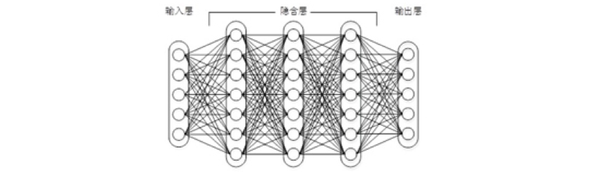
\includegraphics[width=\textwidth]{mlp}
  \caption{上下层神经元全部相连的神经网络——多层感知器}
  \label{fig:mlp}
\end{figure}

显然感知器的层数越多,其刻画现实的能力就越强,不过要让神经网络变深并不容易。
首先随着层数增加,\emph{优化函数越来越容易陷入局部最优解}, 并且这个“陷阱”越来越偏离真正的全局最优。
数据量不大时训练出的深层网络,性能还不如较浅层网络。其次\emph{“梯度消失”现象更加严重},
以sigmoid激活函数为例, 对于幅度为1的信号, 在BP反向传播梯度时,每传递一层,梯度衰减为原来的0.20,
这样层数一多,梯度指数衰减后低层的梯度几乎为0,
找不到合适的迭代方向。最后深层网络将产生海量的参数,
对训练算法和计算机硬件都要求很高.

上述问题都很难解决,所以九十年代, 大家都转而研究浅层学习模型,相继提出了支撑向量机(SVM,Support
Vector Machines)、 Boosting、最大熵方法(如LR,Logistic
Regression)等。这些模型的结构基本上可以看成带有一层隐层节点(如SVM、Boosting),或没有隐层节点(如LR),
此时神经网络的研究相对沉寂.

2006年,加拿大多伦多大学教授、机器学习领域的泰斗Geoffrey Hinton和
他的学生Ruslan Salakhutdinov在《科学》上发表了一篇文章\cite{hinton2006reducing},
开启了深度学习在学术界和工业界的新纪元。
他们利用预训练方法缓解了局部最优解问题, 将隐层数提升到了7.
所谓预训练就是在做有监督学习之前先做无监督学习, 用无监督学习出一些优异的特征
这样再做有监督学习可以得到更好的效果. Hinton使用了逐层优化的
多层限制玻尔兹曼机(Restricted Boltzmann machine, RBM),
又称作Deep Belif Network(DBN). 之后Vincent等\cite{vincent2008extracting}
提出了更好训练的Denoise autoencoder(dA)模型, 也可以做无监督的特征学习.

\section{}

\bibliographystyle{alpha}
\bibliography{ref}

\end{document}

